\chapter{Proposed method}\label{method}

This chapter presents the proposed method, the recommender system uses
user's context to infer the predictions of items.  First, the data
models are defined in order to explain what characteristics (or
information) was used from each model. \\Overall, the post-filtering
approach is applied in order to cover the user's needs in a wider
range of satisfaction and, it is based in the information that users
provide to the recommender system. This chapter describes each
component in the method, as well as its functionality and how is
connected with another components of the method.

\section{Data models} 

The data models was implemented in PostgreSQL database, 
the information in context-aware recommender system was
managed in a scheme of a relational database. Technical support 
about installations of dependencies and the application are 
mentioned in appendix \ref{appendixc}.

\subsection{Restaurant model} 

An effective on-line recommender system must be based upon an
understanding of consumer  preferences and successfully mapping
potential products into the consumer's
preferences\cite{adomavicius2011context}. Pan and
Fesenmaier\cite{pan2006online} argued that this can be achieved
through the understanding of how consumers describe in their own
language a product, a place, and the experience when they are
consuming the product or visiting the place.\\ Traditionally, choosing
a restaurant has been considered as rational behavior where a number
of attributes contribute to the overall usefulness of a restaurant.
For example: food type, service quality, atmosphere of the restaurant,
and availability of information about a restaurant, plays an important
role at different stages in consumer's desitions
making\cite{auty1992consumer}. While food quality and food type have
been perceived as the most important variables for consumers'
restaurant selection, situational and contextual factors have been
found to be important also. Due to this in
Kivela\cite{jack1997restaurant} identifies four types of restaurants:
1) \textit{fine dining/gourmet}, 2) \textit{theme/atmosphere}, 3)
\textit{family/popular}, and 4) \textit{convenience/fast-food}; and
Auty\cite{auty1992consumer} identifies four types of dining out
occasions: 1) \textit{namely celebration}, 2) \textit{social
occasion}, 3) \textit{convenience/quick meal}, and 4) \textit{business
meal}.\\ Taking in account the context, the restaurant model proposed
for context-aware recommender system was definded with 55 attributes
about the restaurants features. An exploration about contents of
models of others works were compared to define the suitable
information into the model. Therefore, the restaurant model is a
binary vector with the following contextual attributes: 1)
\textit{price range}, 2) \textit{payment type}, 3) \textit{alcohol
type}, 4) \textit{smoking area}, 5) \textit{dress code}, 6)
\textit{parking type}, 7) \textit{installations type}, 8)
\textit{atmosphere type}, and 9) \textit{cuisine type}. An example of
restaurant model in the context-aware recommender system is depicted
in figure \ref{fig:restaurantmodel} with some domain values of the
context represented by a binary vector where \textit{1} means that the
restaurant has the property that corresponds to the position value.
Additionally, the restaurant model contains contextual information
such as \textit{users's reviews}, \textit{ratings average}, and
\textit{geographycal location.}\\
\begin{figure*}
\captionsetup{justification=centering,margin=2cm,font=footnotesize}
\centering
\setlength\fboxsep{0pt}
\setlength\fboxrule{0.7pt}
\fbox{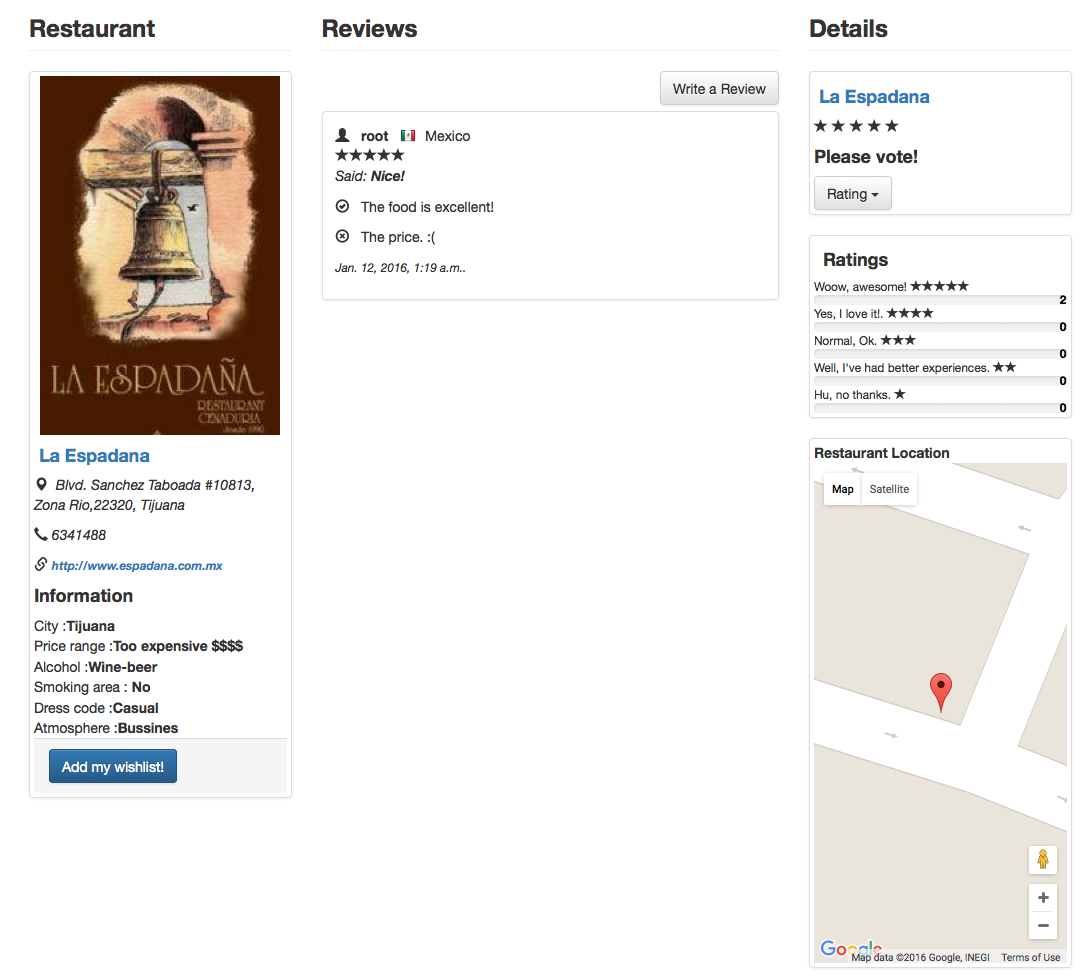
\includegraphics[width=10cm,height=9cm,keepaspectratio]
{img/restaurant-model.png}}
\caption{User interface of the restaurant model.}
\label{fig:restaurantmodel}       
\end{figure*}

\subsubsection{Restuarant data model} \label{datamodelsection}   

The data model in postgreSQL is depicted in the figure
\ref{fig:restaurantmodeldata}, the model contains the restaurant
entity and its attributes. The restaurant entity is related to
\textit{Item entity} in a \textit{``one-to-one"} relation that at the
same time is related to the \textit{RecommenderRule entity} which
specifies some restrictions for item recommendations. A large view of
all the entities related is depicted in the whole scheme refered in
figure \ref{fig:datamodel}.
\begin{figure*}
\captionsetup{justification=centering,margin=2cm,font=footnotesize}
\centering
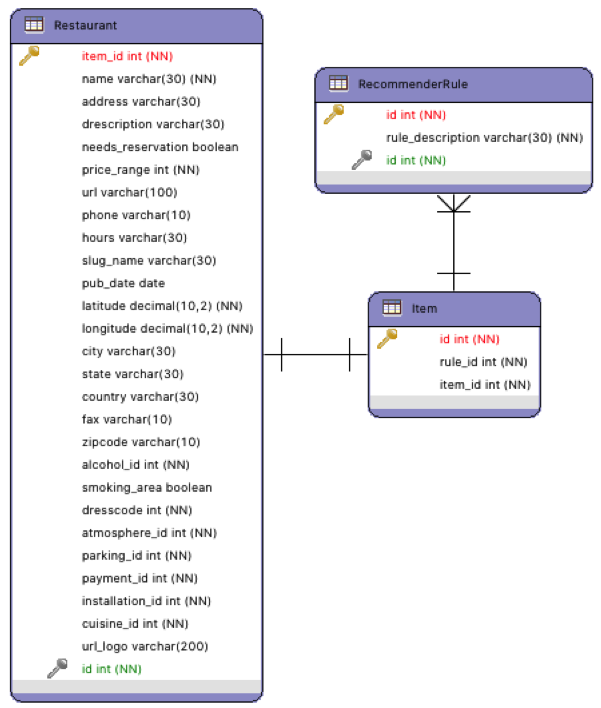
\includegraphics[width=8cm,height=8cm,keepaspectratio]{img/data-resmodel.png}
\caption{The restaurant data model.}
\label{fig:restaurantmodeldata}     
\end{figure*}
Some related entity corresponds to the proposed contextual factors, 
that are defined as following: 
\begin{itemize}
\item \textbf{Price:} \textit{cheap, regular, expensive, too expensive.}
\item \textbf{Payment:} \textit{credit/debit card, cash.}
\item \textbf{Alcohol:} \textit{no alcohol, wine-beer.}
\item \textbf{Smoking area:} \textit{yes, no.}
\item \textbf{Dresscode:} \textit{casual, informal, formal.}
\item \textbf{Installations:} \textit{garden, terrace, indoor, outdoor.}
\item \textbf{Atmosphere:} \textit{relax, familiar, friends, bussines, romantic.}
\item \textbf{Parking:} \textit{no parking, free parking, valet parking.}
\item \textbf{Cuisine:} \textit{japanese, chinese, italian, argentinean,
cantonese, mandarin, mongolian, arabic, greek, spanish, brasilian,
swiss, szechuan, asian, international, steak grill,vegetarian,
natural/healthy/light, traditional mexican, tacos, mediterranean,
middle eastern, american/fast food, gourmet, pizza, bar/beer, tapas
cafe/bar, french, birds, seafood.}
\end{itemize}
The cuisines were defined according the food variety of restaurants in
Tijuana, there are 30 types of cuisines defined in the system. \\
The smoking area is an attribute with boolean value, it
defines if a restaurant has a smoking area in its installation.

\subsection{User model} 

The user's profile is derived from the ratings matrix. Let $U=[u_1,u_2,...u_n]$
the set of all users and $ I=[i_1,i_2,$...$i_n] $ the set of all items, if $R$
represent the ratings matrix,  an element  $R_{u,i}$ represents a user’s rating
$u \in U$  in a item $i \in I$.  The unknown ratings are denoted as $\neq $. The
matrix $R$ can be decomposed into rows vectors, the row vector is denoted as $
\overrightarrow{r_u} $=$[R_{u,1}$...$R_{u,|I|}]$ for every $u \in U$. Therefore,
each row vector represents the ratings of a particular user over the items. Also
denote a set of items rated by a certain user u is denoted as $ I_u = i \in I |
\forall  i: R_{u,i} \neq \emptyset $. This set of items rated represents the
user preferences where for each domain element $R_{u,i} \in [1-5]$ represents
the intensity of the user interest for  the item.\\  
\begin{figure*}
\captionsetup{justification=centering,margin=2cm,font=footnotesize}
\centering
\setlength\fboxsep{0pt}
\fbox{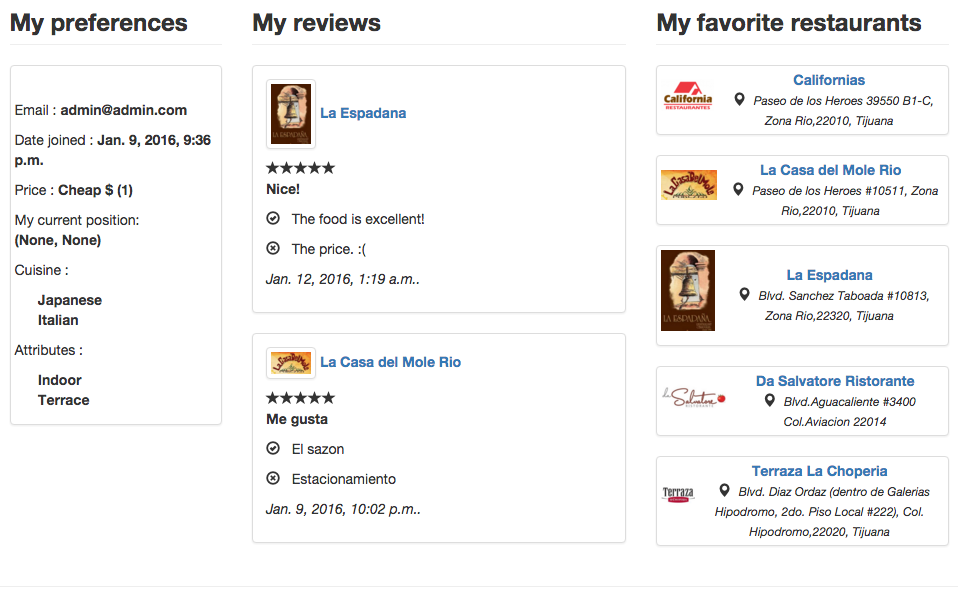
\includegraphics[width=10cm,height=9cm,keepaspectratio]
{img/user-profile.png}}
\caption{Example of user interface for user profile.}
\label{fig:user-profile}      
\end{figure*}
In context-aware recommender system, user profile has contextual
information such as: 1) price range, 2) current location, 3) cuisine
types, 4) attributes or features of restaurants that the user want, 5)
the reviews posted, and 6) the favorite restaurants list. The user
profile is stored in database and it is available for queries request,
and it can be changed by users many times in a session. The
information used to recommendations is the last one register stored.
The user interface is represented in figure \ref{fig:user-profile}.

\subsubsection{User data model} 

The user's data model in postgreSQL is represented in the figure
\ref{fig:datausermodel}, the model involves the entities:
\textit{User, UserProfile, and Friends.} \textit{UserProfile entity}
provides the contextual information of user, \textit{User entity} is
the default model defined in the system and is related to userProfile
for suplies valuable information. 
\begin{figure*}
%\captionsetup{justification=centering,margin=2cm}
\captionsetup{font=footnotesize}
\centering
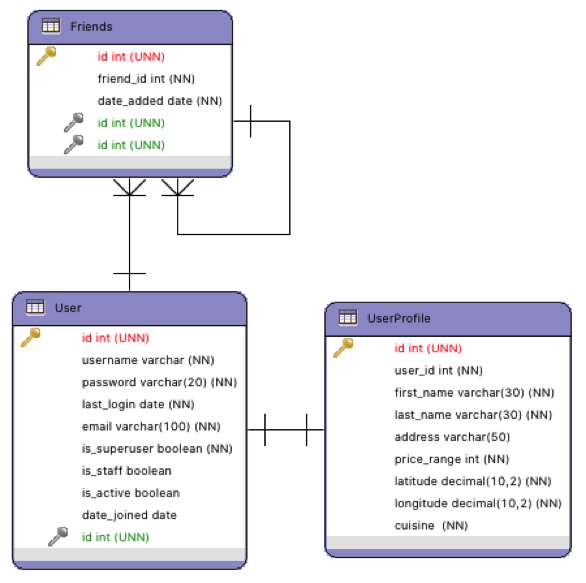
\includegraphics[width=8cm,height=8cm,keepaspectratio]
{img/data-usermodel.png}
\caption{The user data model.}
\label{fig:datausermodel}     
\end{figure*}
The \textit{Friends entity}
represents the social aspect into the userProfile, Friends involves
the users related to the current user taking in account the
preferences of each other. \\The user profile entity is related with: 
price and cuisine are the same that in restaurant model,
attribute groups corresponds to restaurant model mentioned (section
\ref{datamodelsection}). A total of 55 attributes(or characteristics) 
could be contained in user profile, this information is used such as 
contextual information also. The domain values are following:
\begin{itemize}
\item \textbf{Price:} cheap, regular, expensive, too expensive.
\item \textbf{Cuisine:} japanese, chinese, italian, argentinean,
cantonese, mandarin, mongolian, arabic, greek, spanish, brasilian,
swiss, szechuan, asian, international, steak grill,vegetarian,
natural/healthy/light, traditional mexican, tacos, mediterranean,
middle eastern, american/fast food, gourmet, pizza, bar/beer, tapas
cafe/bar, french, birds, seafood.
\item  \textbf{Attribute groups:} Installations, atmosphere, 
parking, payment, smoking area, dresscode, alcohol.
\end{itemize}


\subsection{Relational data model} 

A complete database relational scheme is represented in the figure
\ref{fig:datamodel}. This model involves the whole database for
context-aware recommender system, as well as the entities and
relations among them. \\The context is modeled as a relational
database, each user context is a new register into data table to store
user contexts.\\Contextual information is also stored in the entities:
\textit{Reviews, CurrentLocation, DistancePoi and Ratings.} For
instance, \textit{Reviews entity} describes the user’s opinion about
visited restaurants, this information contributes to have additional
information about recent preferences of diners.\\
\textit{CurrentLocation entity} stores the geographical position of
user to get a \textit{"nearby recommendation"}, the system locates
restaurants around 2 kilometers from the user position, for instance
the system can takes a user position as \textit{latitude:32.529865}
and \textit{longitude: -116.986605}, this information is stored to
calculate distances from this point. The geographical position is
changed frequently, in this manner, it allows the adaptation for each
particular situation of user. \textit{Distance Poi entity} stores the
distances (kilometers) between the user and restaurants, this
information is used to calculate \textit{"nearby recommendation"},
each recommended restaurant ought be over the threshold defined.\\
Finally, \textit{Rating entity} represents the user preferences  
in a vector of ratings that could be increased in time and  
the user's preferences patterns could be changed in time also.
\begin{landscape} 
\begin{figure}[!h] 
\captionsetup{font=footnotesize}
\centering
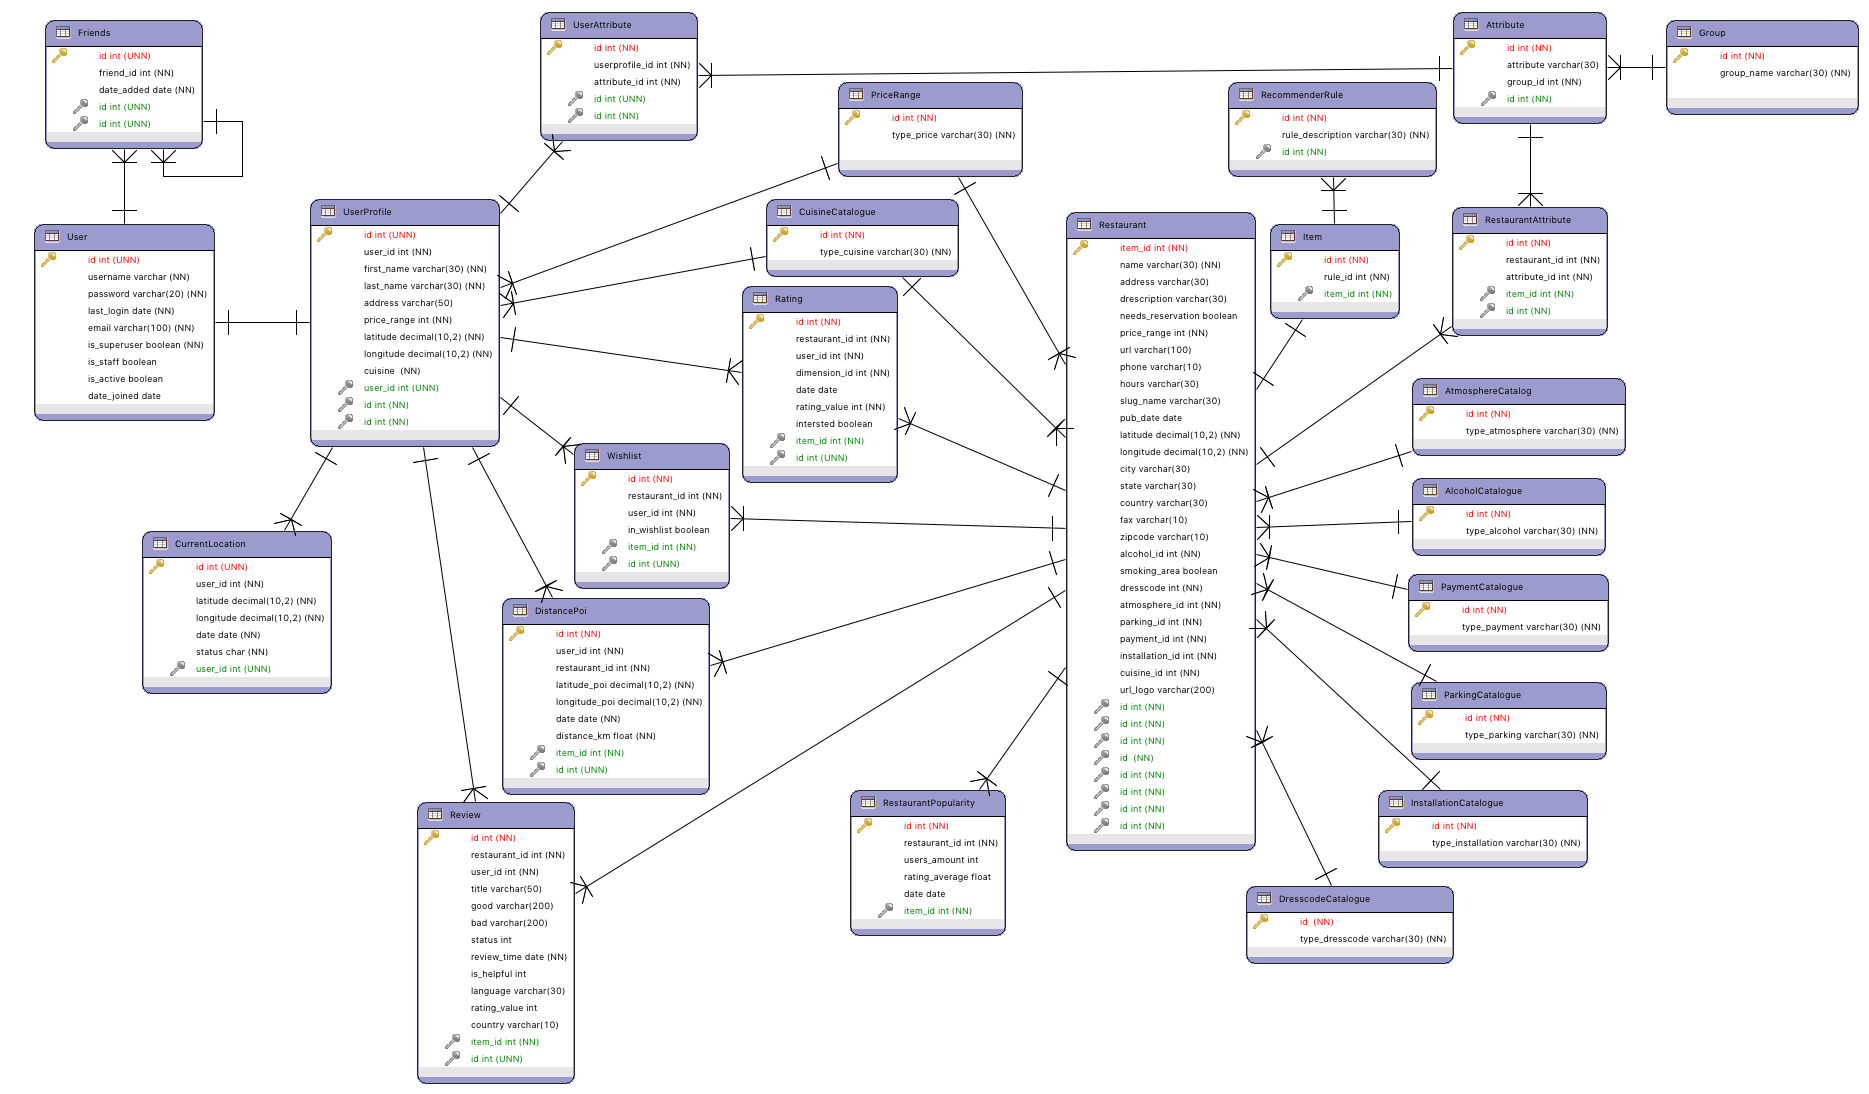
\includegraphics[width=1.3\textwidth]{img/recomet.png}
\caption{The data model of context-aware recommender system.}
\label{fig:datamodel}    
\end{figure}
\end{landscape}

\section{Expert recomendation} 

Fuzzy logic is a methodology that provides a simple way to obtain
conclusions of linguistic data. Is based on the traditional process of
how a person makes decisions based in linguistic information. \\    Fuzzy
logic is a computational intelligence technique that allows to use
information with a high degree of inaccuracy; this is the difference
with the conventional logic that only uses concrete and accurately
information \cite{zedeh1989knowledge}.\\  In this work, fuzzy logic is
used to model fuzzy variables that highligh in the popularity of a
restaurant. The context-aware recommender system has implemented a
fuzzy inference system that represents the expert recommendation. \\   
The expert(fuzzy inference system) generates recommendations when the
recommendation techniques (collaborative filtering, content-based) are
not getting results because of the cold start problem.\\   The fuzzy
inference system proposed has 3 \textbf{input variables} (such as in
previous work realized\cite{garcia2009hybrid}): 1)\textit{rating} is
an average of ratings that has a particular restaurant inside the user
community; the domain of variable is 0 to 5 and contains 2 membership
functions labeled as \textit{low} and \textit{high}(figure
\ref{fig:mf:a}), 2)\textit{price} represents the kind of price that
has a particular restaurant; the domain of variable is 0 to 5 and
contains 2 membership functions labeled as \textit{low} and
\textit{high} (figure \ref{fig:mf:b}), and 3)\textit{votes} is used to
measure how many items have been rated by the current user, i.e., the
participation of the user, if the user has rated few items (less than
10) is not sufficient to make accurate predictions(figure
\ref{fig:mf:c}), the domain of variable is 0 to 10 and contains 2
membership functions labeled as \textit{insufficient} and
\textit{sufficient}. \\ The \textbf{output variable} is
\textit{recommendation}, represents a weight for each restaurant
proposed by the expert considering the inputs mentioned above, the
domain of variable is 0 to 5 and contains 3 membership functions
labeled as \textit{low}, \textit{medium} and \textit{high} (figure
\ref{fig:mf:d}).

\begin{figure}[ht!]
   \captionsetup{font=footnotesize}
   \centering
   %%----primera subfigura----
   \subfloat[]{
        \label{fig:mf:a}
        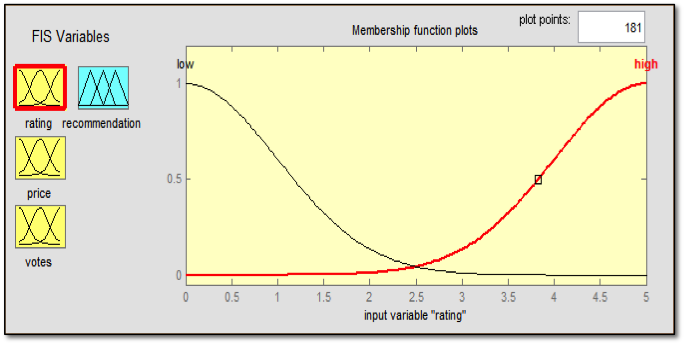
\includegraphics[width=0.42\textwidth]{img/mf-rating.png}}
   \hspace{0.1\linewidth}
   %%----segunda subfigura----
   \subfloat[]{
        \label{fig:mf:b} 
        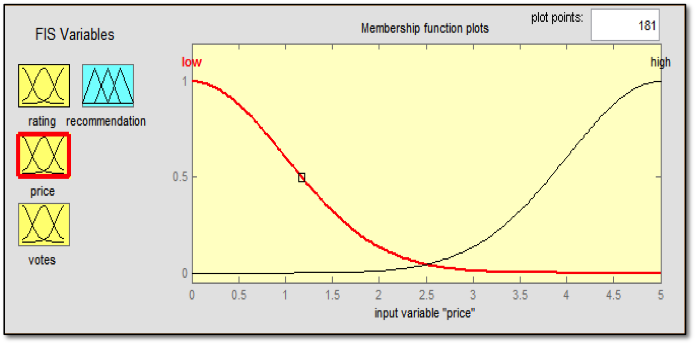
\includegraphics[width=0.42\textwidth]{img/mf-price.png}}\\[20pt]
   %%----tercera subfigura----
   \subfloat[]{
        \label{fig:mf:c} 
        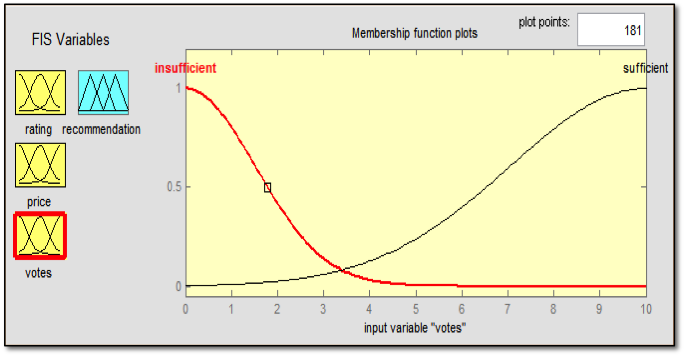
\includegraphics[width=0.42\textwidth]{img/mf-votes.png}}
    \hspace{0.1\linewidth}
   %%----cuarta subfigura----
    \subfloat[]{
        \label{fig:mf:d} 
        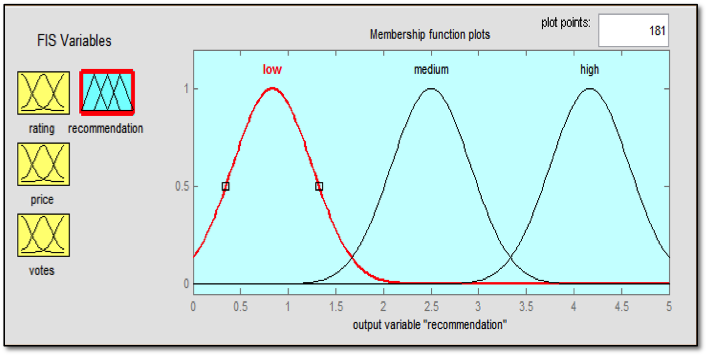
\includegraphics[width=0.42\textwidth]{img/mf-recommendation.png}}
   \caption{The Gaussian membership functions of the expert system.
   }
   \label{fig:mfexpert} 
\end{figure}

The proposed fuzzy inference system(figure \ref{fig:expertfis})
represents the users experience and their knowledge about restaurants.
This factors are considered important for users that visiting a
restaurant. This information is recovered of user profile and
restaurant profile; and the system uses this information to get
weights that influence in the final recommendations. The fuzzy
inference system uses 5 inference rules that involve the variables of
inputs and output. The input variables determine the recommendation
activation; each input variable contains labels as \textit{low} and
\textit{high} that also correspond to memberships functions of
Gaussian type. For the output variable \textit{recommendation} the
labels \textit{low}, \textit{medium}, and \textit{high} are used with
membership functions Gaussian type also. The rules are:
\begin{enumerate} 
\item \textit{If \textbf{rating} is high and \textbf{price} is low then 
\textbf{recommendation} is high.}
\item \textit{If \textbf{rating} is high and \textbf{votes} is sufficient then 
\textbf{recommendation} is high.}
\item \textit{If \textbf{rating} is high and \textbf{votes} is insufficient then 
\textbf{recommendation} is medium.}
\item \textit{If \textbf{rating} is low and \textbf{price} is high and then 
\textbf{recommendation} is low.} 
\item \textit{If \textbf{rating} is low and \textbf{votes} is insufficient then 
\textbf{recommendation} is low.}
\end{enumerate} 
\begin{figure*}
\captionsetup{justification=centering,margin=2cm,font=footnotesize}
\centering
\fbox{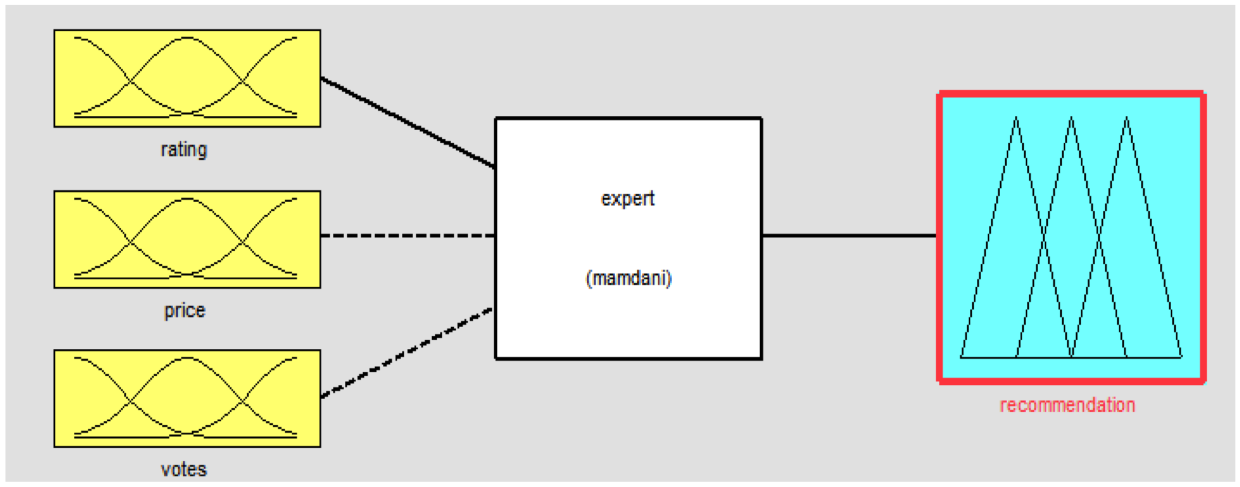
\includegraphics[width=0.70\textwidth]{img/expert.png}}
\caption{Fuzzy Inference System of expert.}
\label{fig:expertfis}      
\end{figure*}

\section{Fuzzy inference system to assing weights} 

The main goal of this fuzzy inference system is to define weights for
each recommendation list. The recommendation technique is based in the
amount of available information stored, so each technique utilizes
this information to provide a list of restaurants as well as a weight
for each one, therefore, these are used for  recommendations if its
weight is upper the threshold.  The fuzzy inference system has inputs
and outputs to infer each list's weight, its variables are depicted in
figure \ref{fig:fis-pesos}.  There are 3 membership functions for
inputs and 3 for outputs. The input variables are:
\textit{userSimilarity, restaurantSimilarity and Participation} and
are depicted in figure \ref{fig:fis-inputs}. The (\ref{fig:fis-inputs}.a) 
and(\ref{fig:fis-inputs}.b) are in a range from 0 to 1 to
define the similarity average among users and restaurants,
respectively. The figure (\ref{fig:fis-inputs}.c) has a range from 0
to 15  to represent the ratings of the user(participation). This
information is stored in the Popularity entity (see figure
\ref{fig:datamodel}). \\
\begin{figure*}
\captionsetup{justification=centering,margin=2cm,font=footnotesize}
\centering
\fbox{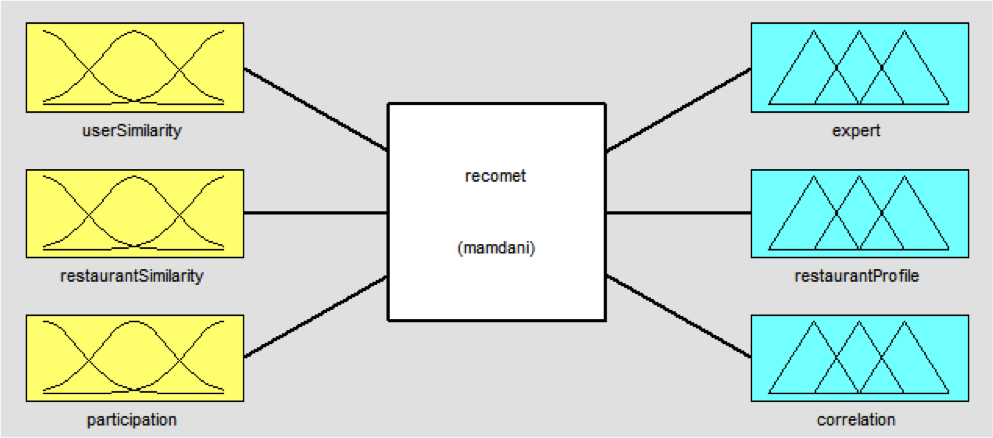
\includegraphics[width=0.70\textwidth]{img/fis-pesos.png}}
\caption{Fuzzy Inference System to assign weights.}
\label{fig:fis-pesos}       
\end{figure*}
By other side, the output variables are: \textit{Expert,
RestaurantProfile and Correlation}, these are depicted in figure
\ref{fig:fis-outputs}. The figure (\ref{fig:fis-outputs}.a) represents
the weight for expert recommendation list, figure (\ref{fig:fis-outputs}.b) 
represents the weight of the content-based list and figure
(\ref{fig:fis-outputs}.c) represents the weight of collaborative
recommendation list, their membership functions are in a range from 0
to 1 to get the value.
\begin{figure}[ht!]
   \captionsetup{font=footnotesize}
   \centering
   %----primera subfigura----
   \subfloat[]{
        \label{fig:mf:a}
        \fbox{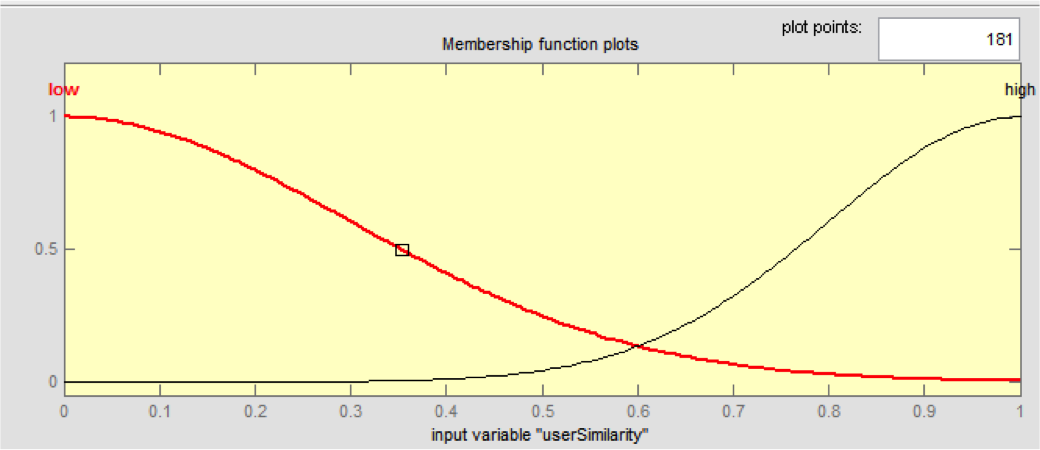
\includegraphics[width=0.42\textwidth]{img/usersimilarity.png}}}
   \hspace{0.1\linewidth}
   %%----segunda subfigura----
   \subfloat[]{
        \label{fig:mf:b} 
        \fbox{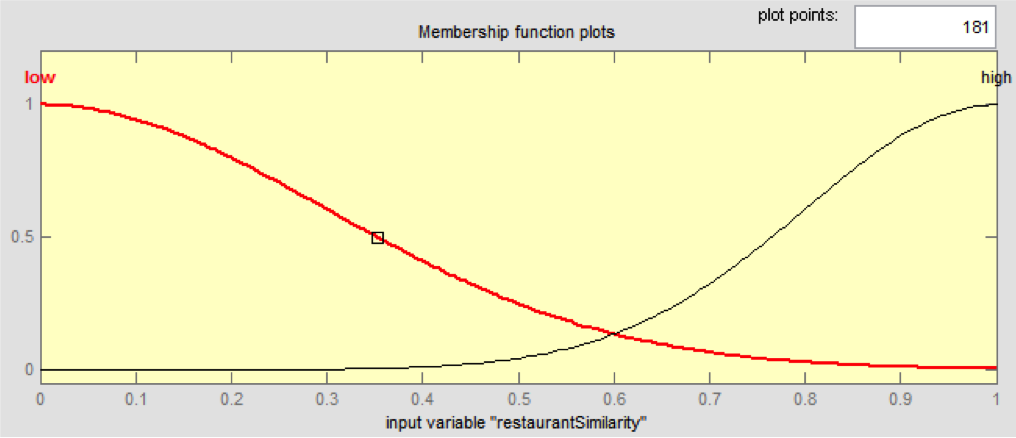
\includegraphics[width=0.42\textwidth]{img/restaurantsimilarity.png}}}\\% 
   %%----tercera subfigura----
   \subfloat[]{
        \label{fig:mf:c} 
        \fbox{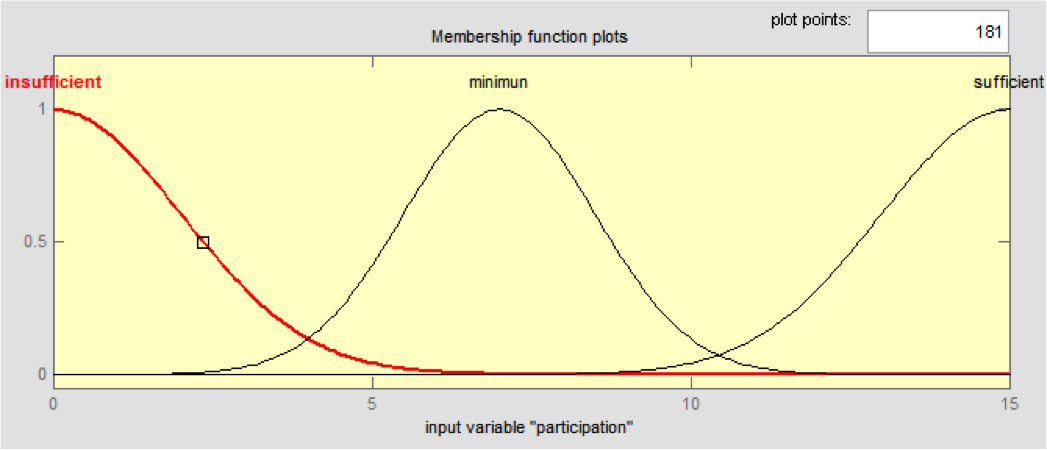
\includegraphics[width=0.42\textwidth]{img/participation.png}}}
        %\hspace{0.1\linewidth}
   \caption{The Gaussian membership functions of input variables.
   }
   \label{fig:fis-inputs} 
\end{figure}
\begin{figure}[ht!]
   \captionsetup{font=footnotesize}
   \centering
   %%----primera subfigura----
    \subfloat[]{
        \label{fig:mf:d} 
        \fbox{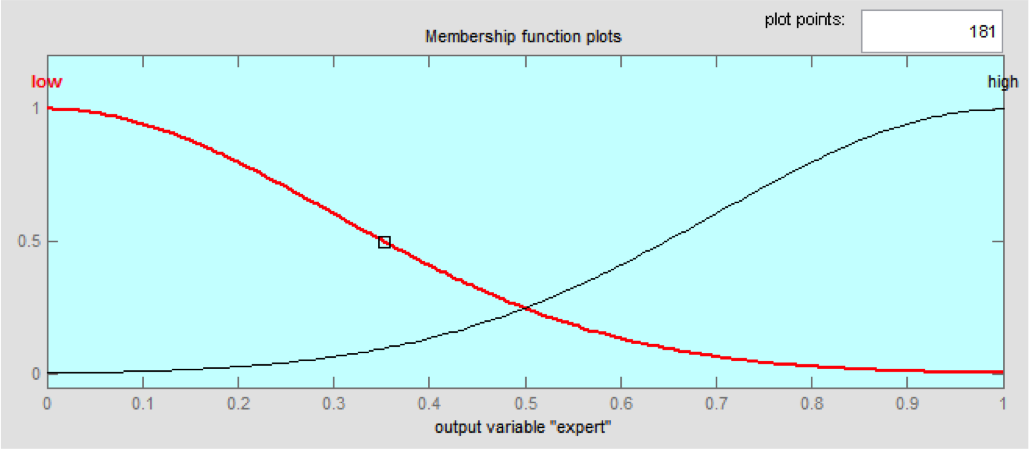
\includegraphics[width=0.42\textwidth]{img/expert-mf.png}}}%\\ %[20pt]
        \hspace{0.1\linewidth}
      %%----segunda subfigura----
    \subfloat[]{
        \label{fig:mf:d} 
        \fbox{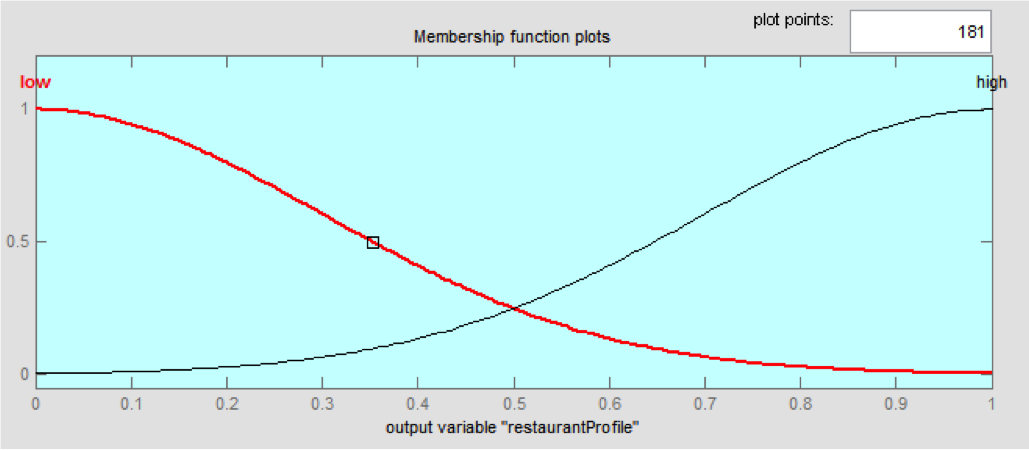
\includegraphics[width=0.42\textwidth]{img/restaurantprofile-mf.png}}}\\
     %%----tercera subfigura----
    \subfloat[]{
        \label{fig:mf:d} 
        \fbox{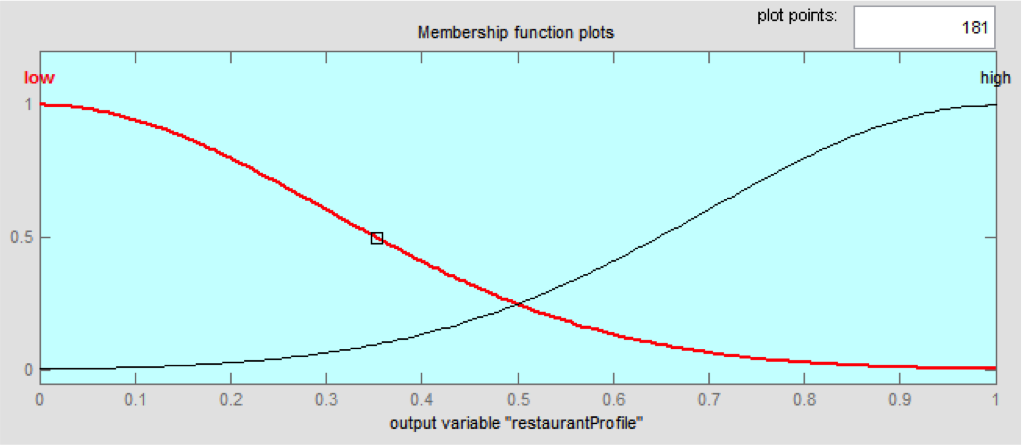
\includegraphics[width=0.42\textwidth]{img/correlation-mf.png}}}%\\ %[20pt]
   \caption{The Gaussian membership functions of output variables.
   }
   \label{fig:fis-outputs} 
\end{figure}
Taking in account the input variables, the rules utilized to infer the 
output values are following:
\begin{enumerate} 
\item \textit{If \textbf{userSimilarity} is low and 
\textbf{restaurantSimilarity} is low and \textbf{participation} 
is insufficient then \textbf{expert} is high, \textbf{restaurantProfile} 
is low, \textbf{correlation} is low.}
\item \textit{If \textbf{userSimilarity} is low and 
\textbf{restaurantSimilarity} is low and \textbf{participation} 
is sufficient then \textbf{expert} is low, \textbf{restaurantProfile} 
is low, \textbf{correlation} is high.}
\item \textit{If \textbf{userSimilarity} is low and 
\textbf{restaurantSimilarity} is low and \textbf{participation} 
is minimun then \textbf{expert} is low, \textbf{restaurantProfile} 
is low, \textbf{correlation} is high.}
\item \textit{If \textbf{userSimilarity} is low and 
\textbf{restaurantSimilarity} is high and \textbf{participation} 
is insufficient then \textbf{expert} is low, \textbf{restaurantProfile} 
is high, \textbf{correlation} is low.}
\item \textit{If \textbf{userSimilarity} is low and 
\textbf{restaurantSimilarity} is high and \textbf{participation} 
is minimun then \textbf{expert} is low, \textbf{restaurantProfile} i
s high, \textbf{correlation} is low.}
\item \textit{If \textbf{userSimilarity} is low and 
\textbf{restaurantSimilarity} is high and \textbf{participation} 
is sufficient then \textbf{expert} is low, \textbf{restaurantProfile} 
is high, \textbf{correlation} is low.}
\item \textit{If \textbf{userSimilarity} is high and 
\textbf{restaurantSimilarity} is low and \textbf{participation} 
is insufficient then \textbf{expert} is low, \textbf{restaurantProfile} 
is low, \textbf{correlation} is high.}
\item \textit{If \textbf{userSimilarity} is high and 
\textbf{restaurantSimilarity} is low and \textbf{participation} 
is minimun then \textbf{expert} is low, \textbf{restaurantProfile} 
is low, \textbf{correlation} is high.}
\item \textit{If \textbf{userSimilarity} is high and 
\textbf{restaurantSimilarity} is low and \textbf{participation} 
is sufficient then \textbf{expert} is low, \textbf{restaurantProfile} 
is low, \textbf{correlation} is high.}
\item \textit{If \textbf{userSimilarity} is high and 
\textbf{restaurantSimilarity} is high and \textbf{participation} 
is insufficient then \textbf{expert} is low, \textbf{restaurantProfile} 
is low, \textbf{correlation} is high.}
\item \textit{If \textbf{userSimilarity} is high and 
\textbf{restaurantSimilarity} is high and \textbf{participation} 
is sufficient then \textbf{expert} is low, \textbf{restaurantProfile} 
is low, \textbf{correlation} is high.}
\item \textit{If \textbf{userSimilarity} is high and 
\textbf{restaurantSimilarity} is high and \textbf{participation} 
is minimun then \textbf{expert} is low, \textbf{restaurantProfile} 
is low, \textbf{correlation} is high.}
\end{enumerate} 
At the end, a \textit{weighted average} allows to get predictions for
each restaurant in the list of recommendations. In this way, for
instance if the \textbf{expert} has a weight of \textbf{0.5}, the
\textbf{restaurantProfile} is \textbf{0.8} and the
\textbf{correlation} is \textbf{0.6}, the system uses these weights to
calculate the final prediction for a particular restaurant using the
formula of the weighted average:
\begin{equation}\label{eq:prediction}
\displaystyle prediction_{i} = {(0.5 * 4.0) + ( 0.8 * 5) + (0.6 * 4.5)
\over (0.5 + 0.8 + 0.6)}
\end{equation}
The prediction corresponds the final value of recommendation for the
item, and is used to include it or exclude it of the list of
recommendation if is not over the threshold. So, for this case, the
prediction is \textbf{4.57}, it means that this restaurant will be in the
recommendation list of the user, subsequently, the recommendations
list will be contextualized.

\section{Contextual recommendation} 

The interface of the system(figure \ref{fig:context}) allows to
collect contextual information such as type of price, restaurant's
attributes, type of cuisine and geographical location. \\ 
The context-aware recommender system uses post-filtering paradigm, 
then the contextual information is used for adjust the final 
recommendations list. For example, geographical location is used to get restaurants
around 2 kilometers of distance, next, the list of nearby restaurants
is displayed for the user.\\  
\begin{figure*}
\captionsetup{justification=centering,margin=2cm,font=footnotesize}
\centering
\fbox{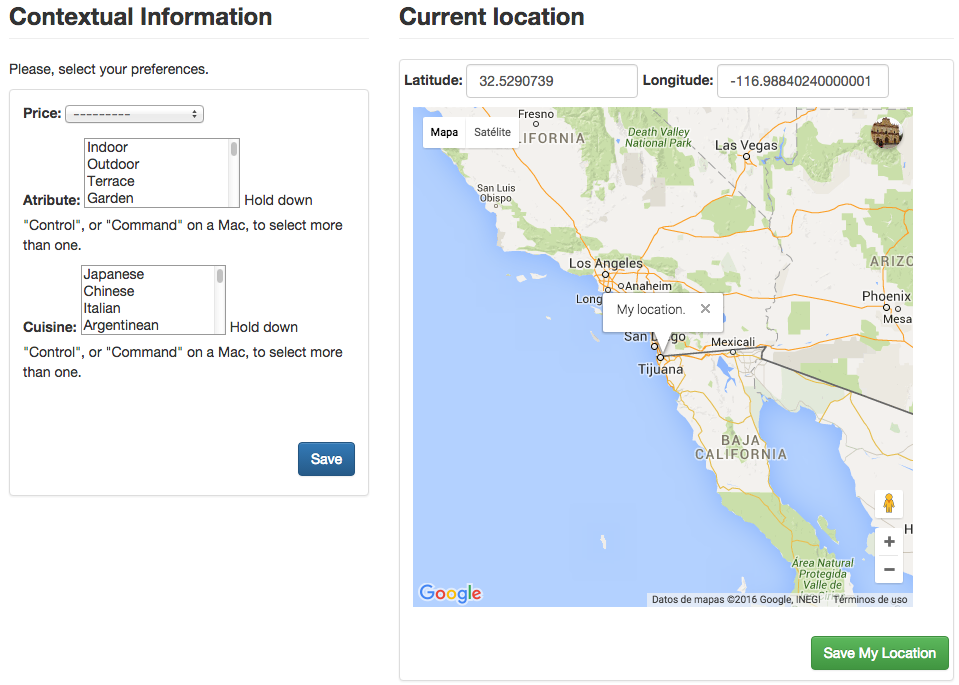
\includegraphics[width=0.60\textwidth]{img/context.png}}
\caption{System interface to collect contextual information.}
\label{fig:context}   
\end{figure*}
If context-aware recommender system
considers another attributes as type of price and type of cuisine
preferred by the user, the system gets restaurants matched in the
context especified by the user in this time. 
\begin{figure*}
\captionsetup{font=footnotesize}
\centering
\fbox{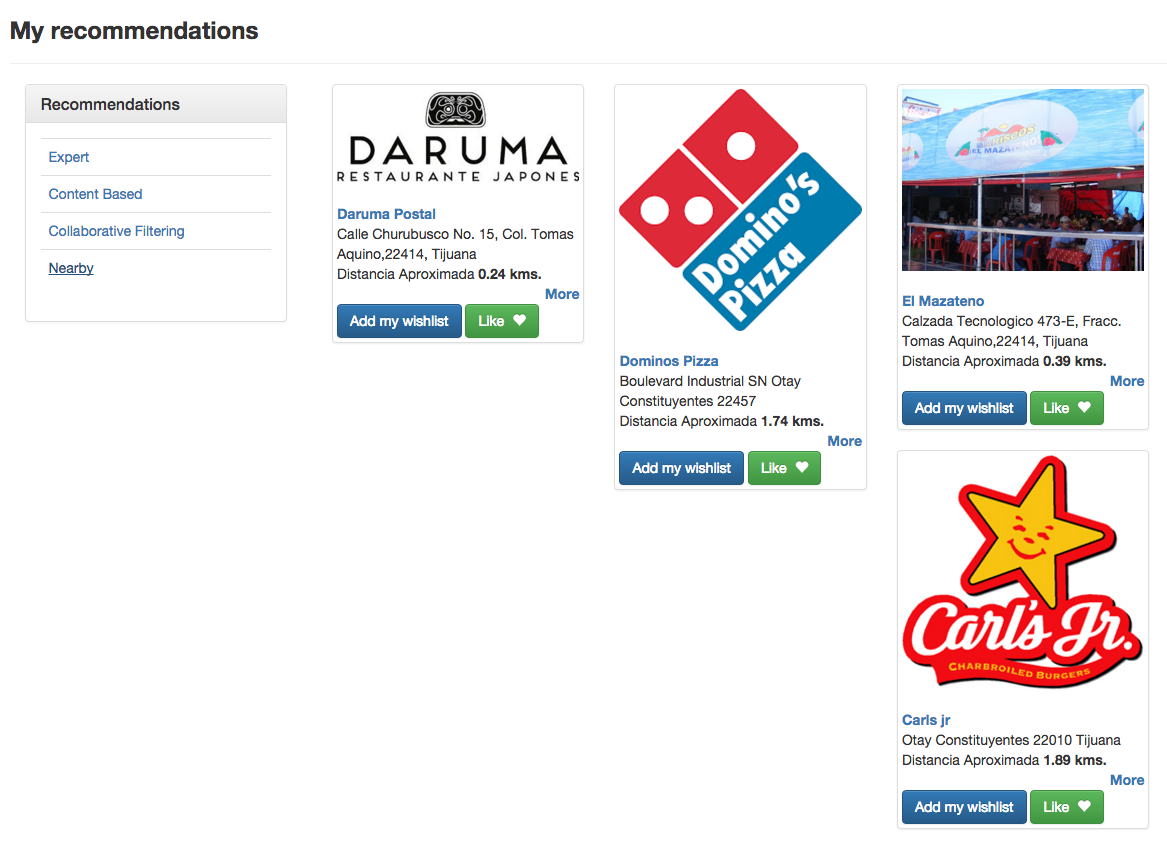
\includegraphics[width=0.60\textwidth]{img/recom.png}}
\caption{System inferface of recommendations for the user.}
\label{fig:recom}    
\end{figure*}
In the attributes box,
the user can chose any preference about what things are importants to
select a restaurant. The features are collected from the dataset of
Tijuana restaurants. In the cuisine box, the user choosen his/her
favorite cuisine, it can be one or more cuisines such as in attributes 
also. 
The context changes constantly, indeed, the users migh change 
it many times such as them wish.\\ 
After the post-filtering, the system displays the  recommended
restaurants according the information provides by the user. The
context-aware recommender system contains four techniques to display
recommendations. The interface in figure \ref{fig:recom} shows
recommendations: \textit{1) Expert, 2) Content-based, 3) Collaborative
filtering and 4) Nearby.} Each one was explained above, except the
nearby recommendations. For nearby recommendations the system
calculates the approximate distance between the current geographical
location of the user and the available restaurants in the area.  The
threshold is 2 kilometers around the user position to determine what
restaurants will be recommended. The geographical position is
obtained throught Google maps services.


\section{Methodology} 

The scheme of proposed method is depicted in the figure
\ref{fig:archit}. In the first part, the three techniques of
recommendations are suplied by the rating matrix. \\
Ratings matrix makes that \textbf{fuzzy inference system} can obtain
the inputs values to calculate the output value. 
\begin{figure*}
\captionsetup{font=footnotesize}
\centering 
%\fbox{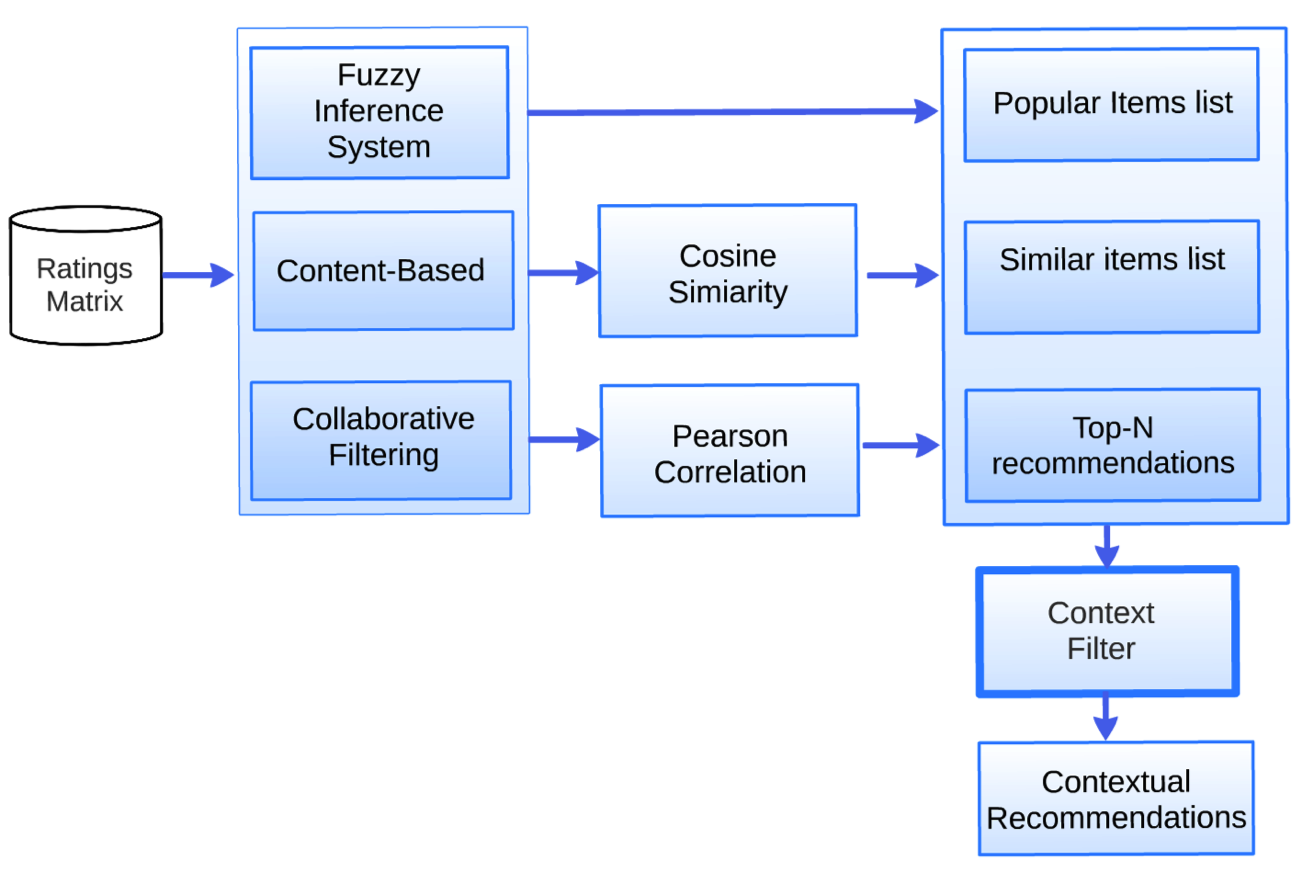
\includegraphics[width=10cm,height=10cm,keepaspectratio]{img/archit.png}}
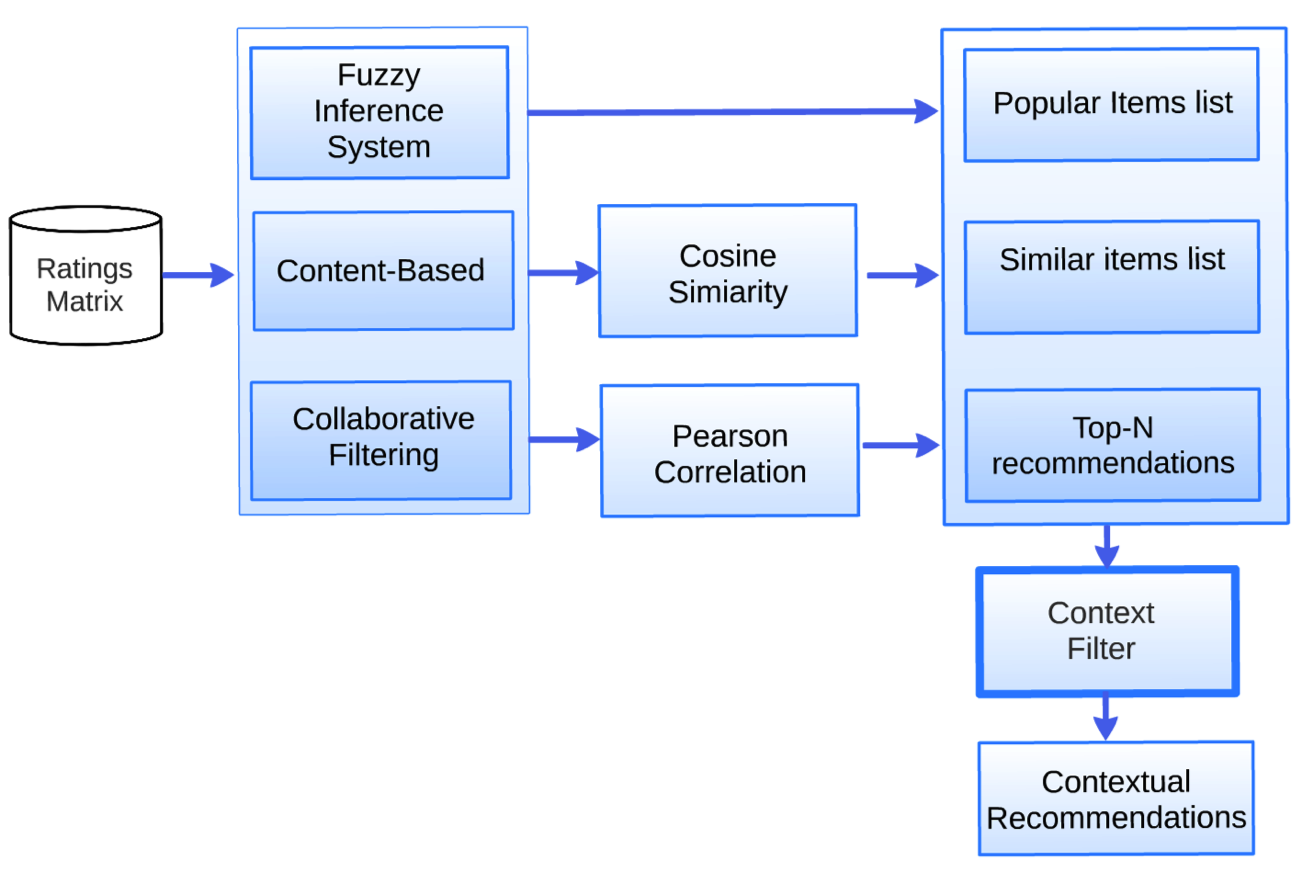
\includegraphics[width=10cm,height=10cm,keepaspectratio]{img/archit.png}
\caption{Scheme of the proposed method.}
\label{fig:archit}  
\end{figure*}
\textbf{Content-based} 
utilizes the rating matrix and user profiles to compare the
similarity among the restaurants through cosine similarity measure.
\textbf{Collaborative filtering} is based in user profiles content in
ratings matrix, using Pearson correlation calculates the similarity
among the users, subsequently, a list of neighbors is obtained to use
their preferences to calculate predictions.\\
The second part shows the recommendation lists for the user. Later,
the recommendation lists are reduced when filter of context is applied,
i.e., the recommendations are adjusted for the user current context.
Finally, the contextual recommendations list is displayed in the user
interface (figure \ref{fig:recom}).






